\documentclass[11pt,a4paper]{article}

\usepackage[T1]{fontenc}
\usepackage[utf8]{inputenc}
\usepackage{lmodern}
\usepackage[margin=1.8cm]{geometry}
\usepackage{amsmath,amssymb,bm}
\usepackage{graphicx}
\usepackage{wrapfig}
\usepackage{booktabs}
\usepackage{caption}
\usepackage{xcolor}
\usepackage[hidelinks]{hyperref}
\usepackage{enumitem}
\usepackage{titlesec}

\definecolor{accent}{HTML}{2A6FD6}
\titleformat*{\section}{\large\sffamily\bfseries\color{accent}}
\titleformat*{\subsection}{\normalsize\sffamily\bfseries\color{accent}}
\titlespacing*{\section}{0pt}{8pt}{3pt}
\titlespacing*{\subsection}{0pt}{5pt}{1pt}
\setlength{\textfloatsep}{8pt plus 2pt minus 2pt}
\setlength{\intextsep}{8pt plus 2pt minus 2pt}
\setlength{\abovecaptionskip}{4pt}

\graphicspath{{../figures/}{../figures/analysis_report/}}
\captionsetup{font=small,labelfont=bf}
\setlist{itemsep=1pt,topsep=3pt}
\setlength{\parskip}{3pt}
\setlength{\parindent}{0pt}

\newcommand{\R}{\mathbb{R}}
\newcommand{\E}{\mathbb{E}}
\newcommand{\Var}{\mathrm{Var}}
\newcommand{\Cov}{\mathrm{Cov}}
\newcommand{\N}{\mathcal{N}}
\newcommand{\rhat}{\hat r}

\begin{document}

%% ---------------------------------------------------------------- cover page
\begin{titlepage}
\centering\sffamily
\vspace*{\fill}
{\color{accent}\huge Data Science Lab A1 - Final report\par}
\vspace{0.4cm}
{\color{accent}\Large Movie rating prediction with Bayesian factorization machines\par}
\vspace{2cm}
{\Large Quentin Revillon, Vincent Ami\par}
\vspace{0.3cm}
{\large Group 40, La piscine\par}
\vspace{1.2cm}
{DataLab A1, Master IASD\par}
\vspace{1cm}
{\Large October 2026\par}
\vspace*{\fill}
%% short contents
\begin{minipage}{0.7\linewidth}
\small
\setcounter{tocdepth}{1}
\renewcommand{\contentsname}{\normalsize Contents}
\tableofcontents
\end{minipage}
\vspace{1cm}
\end{titlepage}

%% ================================================================ 1
\section{Problem, data and protocol}

The ratings form a matrix $R \in \R^{n_u \times n_i}$ with $n_u = 610$ users and $n_i = 4980$ movies,
ratings in $\{0.5, 1, \dots, 5\}$. $\Omega$ is the set of observed pairs $(u,i)$, $\Omega_u$ the movies
rated by $u$ and $\Omega_i$ the users who rated $i$. Train and test each hold $31\,598$ ratings (density
$1.04\%$). A model outputs $\rhat_{ui}$ for every pair and is scored by
$\mathrm{RMSE} = \big(\frac{1}{|\Omega_{\text{eval}}|}\sum_{(u,i)\in\Omega_{\text{eval}}} (r_{ui}-\rhat_{ui})^2\big)^{1/2}$.
All predictions are clipped to $[0.5, 5]$.

Sections 2 and 3 follow a first protocol (A): hyperparameters are chosen by 5-fold cross-validation on the
observed entries of the train set (each fold fits on $80\%$ and validates on $20\%$, fixed seed), then the chosen
model is refitted on the whole train set and scored once on the test set. Section 4 follows a second protocol (B).
The platform fits on train $\cup$ test, twice as many ratings as the train set, and we found that the optimal
rank depends on the amount of data (Section~\ref{sec:protocol}). We therefore cross-validate on train $\cup$ test (5 folds,
same seed). The out-of-fold predictions of protocol B are also the training set of the stacking models.
On the platform, the score has stayed about $0.009$ below this CV score.

Besides NumPy and SciPy, we used \texttt{myfm} (Gibbs sampler of the Bayesian factorization machine),
scikit-learn (gradient boosting) and Optuna (hyperparameter search).

%% ================================================================ 2
\section{Building the baseline}

\subsection{Rating biases}
The model $\rhat_{ui} = \mu + b_u + b_i$, where $\mu$ is the mean rating, solves
\[
\min_{b} \sum_{(u,i)\in\Omega} (r_{ui} - \mu - b_u - b_i)^2 + \lambda_u \lVert b_u\rVert^2 + \lambda_i \lVert b_i\rVert^2
\]
by alternating exact ridge updates, e.g.\ $b_i = \sum_{u\in\Omega_i}(r_{ui}-\mu-b_u)/(\lambda_i+|\Omega_i|)$.
Cross-validation gives $\lambda_u = 5$ and $\lambda_i = 3$, so the bias of a movie rated once is divided by 4.

\subsection{Matrix factorization}
We add a low-rank interaction, $\rhat_{ui} = \mu + b_u + b_i + \langle U_u, V_i\rangle$ with
$U \in \R^{n_u\times k}$ and $V \in \R^{n_i\times k}$ (the course writes $R \approx U I^\top$), and minimize the
squared error plus $\lambda_U\lVert U\rVert^2 + \lambda_V\lVert V\rVert^2 + \lambda_b(\lVert b_u\rVert^2+\lVert b_i\rVert^2)$.
We compared full-batch gradient descent with momentum and ALS, whose steps are row-wise ridge regressions.
On the same cost, ALS reaches the same validation RMSE as gradient descent about five times faster (3.4\,s
against 17\,s). The model without $\mu$ and biases, $\rhat_{ui} = \langle U_u, V_i\rangle$, is much worse
(test $0.979$): with about 52 ratings per user, a rank-$k$ model has to spend its capacity on the mean levels.
An Optuna search (30 trials, separate $\lambda_U, \lambda_V, \lambda_b$) drives $\lambda_U$ to $54$ and the rank
to 2, which switches the factors off: the model falls back to the biases.

\subsection{Neighbourhood models}
The item kNN corrects the bias residuals $e_{uj} = r_{uj} - \mu - b_u - b_j$:
\[
\rhat_{ui} = \mu + b_u + b_i + \frac{\sum_{j \in N_k(i;u)} s_{ij}\, e_{uj}}{\delta + \sum_{j\in N_k(i;u)} |s_{ij}|},
\qquad s_{ij} = \frac{n_{ij}}{n_{ij}+\beta}\,\rho_{ij},
\]
where $N_k(i;u)$ are the $k = 20$ movies rated by $u$ most similar to $i$, $\rho_{ij}$ is the Pearson correlation
of the residuals over the $n_{ij}$ common users, $\beta = 100$ shrinks similarities computed on few users and
$\delta = 0.5$ damps the correction when the neighbours are weak. We also tried the user kNN and Koren's
global neighbourhood model, where the weights $w_{ij}$ are learnt instead of set to $s_{ij}$.

\subsection{Results}
No model beats the biases by more than $0.005$ on the test set (Table~\ref{tab:baselines}), less than the
fold-to-fold standard deviation of the CV RMSE ($\approx 0.006$). At $1\%$ density, a movie has 3 training
ratings on median: the user and movie offsets are well estimated, the interaction term is not. Point
estimates of $U$ and $V$ either overfit or, once regularized enough, vanish. We keep $\mu + b_u + b_i$ as the baseline.

\begin{table}[h]
\centering\small
\begin{tabular}{lccc}
\toprule
Model (protocol A) & CV RMSE (train) & Test RMSE & Test accuracy \\
\midrule
Global mean $\mu$                                   & --     & 1.0369 & 0.129 \\
\textbf{Biases} ($\lambda_u=5$, $\lambda_i=3$)      & 0.8829 & \textbf{0.8744} & 0.244 \\
MF with biases, gradient descent ($k=50$, $\lambda=10$) & 0.8830 & 0.8723 & 0.248 \\
MF with biases, ALS + Optuna ($k=2$)                & 0.8831 & 0.8744 & 0.245 \\
User kNN ($k=40$)                                   & 0.8817 & 0.8716 & 0.246 \\
Item kNN ($k=20$, $\beta=100$, $\delta=0.5$)        & 0.8790 & 0.8692 & 0.249 \\
Koren, learnt weights ($k=200$)                     & 0.8800 & 0.8704 & 0.251 \\
\midrule
BPMF with biases, $\alpha = 2$ (paper)              & 0.8820 & 0.8690 & 0.248 \\
BPMF with biases, $\alpha = 1.5$ (CV)               & 0.8776 & 0.8653 & 0.247 \\
\bottomrule
\end{tabular}
\caption{Protocol A. Accuracy is the share of predictions that round to the exact half-star. The standard
deviation of the CV RMSE across folds is about $0.006$ for every model.}
\label{tab:baselines}
\end{table}

%% ================================================================ 3
\section{Bayesian probabilistic matrix factorization (BPMF)}
Salakhutdinov and Mnih (ICML 2008) replace the point estimate of $(U, V)$ by an average over the posterior,
which integrates the regularization instead of tuning it. We use the variant with biases, where the bias is
appended to each latent vector, $U_u \leftarrow (U_u, b_u)$ and $V_i \leftarrow (V_i, b_i)$, of dimension
$D = k + 1$.

The likelihood, priors and hyperpriors are
\[
r_{ui} \mid U, V \sim \N\!\big(\mu + \langle U_u, V_i\rangle,\ \alpha^{-1}\big), \qquad
U_u \mid \mu_U, \Lambda_U \sim \N(\mu_U, \Lambda_U^{-1}), \qquad V_i \mid \mu_V, \Lambda_V \sim \N(\mu_V, \Lambda_V^{-1}),
\]
\[
p(\mu_U, \Lambda_U) = \N\!\big(\mu_U \mid \mu_0, (\beta_0\Lambda_U)^{-1}\big)\ \mathcal{W}(\Lambda_U \mid W_0, \nu_0),
\quad\text{and the same for } (\mu_V, \Lambda_V),
\]
with the paper's values $\mu_0 = 0$, $\beta_0 = 2$, $W_0 = I_D$, $\nu_0 = D$. The noise precision $\alpha$ is the
only fixed hyperparameter; $\alpha^{-1/2}$ is the standard deviation of a rating around the model.

\subsection{Gibbs sampling}
The Gauss-Wishart prior is conjugate, so every block has a closed-form conditional posterior. Given $U$, with
mean $\bar U$ and empirical covariance $\bar S$ over its $n_u$ rows, $(\mu_U, \Lambda_U)$ is Gauss-Wishart with
\[
\beta^* = \beta_0 + n_u,\quad \nu^* = \nu_0 + n_u,\quad
\mu^* = \frac{\beta_0\mu_0 + n_u\bar U}{\beta_0 + n_u},\quad
(W^*)^{-1} = W_0^{-1} + n_u\bar S + \frac{\beta_0 n_u}{\beta_0+n_u}(\mu_0-\bar U)(\mu_0-\bar U)^\top .
\]
Given $V$ and the hyperparameters, the users are independent Gaussians:
\[
U_u \mid \cdot \sim \N\!\big(m_u, A_u^{-1}\big),\qquad
A_u = \Lambda_U + \alpha\!\sum_{i\in\Omega_u}\! V_i V_i^\top,\qquad
m_u = A_u^{-1}\Big(\Lambda_U\mu_U + \alpha\!\sum_{i\in\Omega_u}\!(r_{ui}-\mu)\,V_i\Big).
\]
The mean $m_u$ is a ridge regression of the user's ratings on the movie vectors, with the learnt prior
$(\mu_U, \Lambda_U)$ in place of a hand-tuned $\lambda$; the movies are symmetric. One Gibbs iteration draws
$(\mu_U,\Lambda_U)$, then all $U_u$, then $(\mu_V,\Lambda_V)$ and all $V_i$. After a burn-in of 20 iterations,
the prediction is the average of the samples' predictions,
$\rhat_{ui} = \frac{1}{T}\sum_{t=1}^{T}\big(\mu + \langle U^{(t)}_u, V^{(t)}_i\rangle\big)$, a Monte Carlo
estimate of the posterior mean. The chain starts from a few ALS iterations, as the paper starts from the MAP
solution; 2, 10 or 30 of them give the same CV RMSE within $0.003$.

\subsection{Results}
\begin{wrapfigure}{r}{0.47\linewidth}
\vspace{-12pt}
\centering
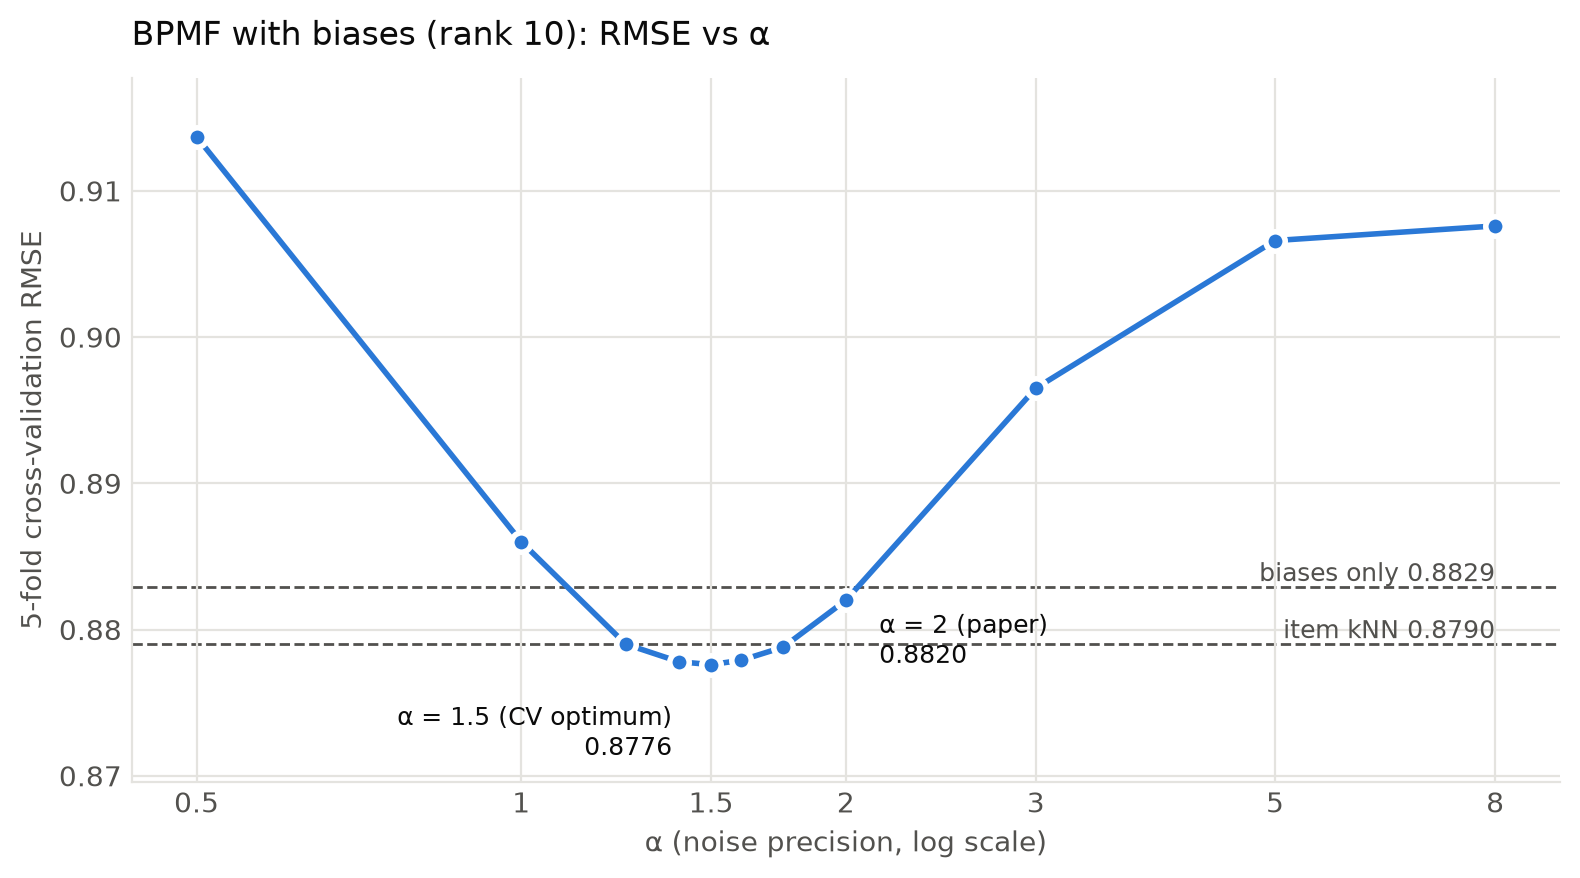
\includegraphics[width=\linewidth]{bpmf_alpha.png}
\caption{BPMF with biases, rank 10: 5-fold CV RMSE on the train set as a function of the noise precision $\alpha$.}
\label{fig:alpha}
\vspace{-8pt}
\end{wrapfigure}
The averaging is what makes the model work. On a validation fold, the RMSE of a single sample rises from
$0.93$ to $1.0$ as the chain explores, while the RMSE of the running average decreases to $0.878$: each sample
overfits, their average does not. Figure~\ref{fig:alpha} shows the CV RMSE as a function of $\alpha$. With
the paper's $\alpha = 2$ (noise standard deviation $0.71$), BPMF only matches the biases. The optimum
$\alpha = 1.5$ (standard deviation $0.82$) is closer to the error level actually reached ($0.88$ in CV),
gains $0.0044$ in CV and gives the best test RMSE of protocol A ($0.8653$, Table~\ref{tab:baselines}).
We also sampled $\alpha$ in the Gibbs chain, with a conjugate $\mathrm{Gamma}(1,1)$ prior. The CV RMSE is the
same ($0.8780$), but $\alpha$ drifts from $1.45$ to $2.3$: it is fitted to the training residuals of the
current sample, which shrink as the chain overfits. A fixed $\alpha$ acts as a regularization that the sampled
one loses.

%% ================================================================ 4
\section{Bayesian factorization machines}
A factorization machine (Rendle, 2010) predicts from a sparse feature vector $x$:
\[
\rhat(x) = w_0 + \sum_j w_j x_j + \sum_{j<l} \langle v_j, v_l\rangle\, x_j x_l .
\]
With $x$ equal to the one-hot of $u$ concatenated with the one-hot of $i$, this is exactly BPMF with biases.
The Bayesian FM (Freudenthaler, Schmidt-Thieme and Rendle, 2011) keeps the same Gibbs scheme and differs from
BPMF in three ways: any feature can enter $x$; each feature group (users, movies, genres, \dots) has its own
Gaussian prior with Normal-Gamma hyperpriors on its mean and diagonal precision, instead of a full Wishart;
and $\alpha$ is sampled. Our feature vector adds two kinds of information to the two one-hot blocks.
The implicit feedback puts in the user block the movies rated by $u$, each with value $|\Omega_u|^{-1/2}$ as in
SVD++, and in the movie block the users who rated $i$, with value $|\Omega_i|^{-1/2}$. These sets are built from
the training ratings only. The side information is the genres (multi-hot) and the release decade (one-hot) of
the movie. The genre file first provided was aligned with only 648 of the 4980 columns; the corrected file
reduces the CV RMSE of the full model by $0.020$ and its test RMSE from $0.8552$ to $0.8403$.

\subsection{Results and change of protocol}\label{sec:protocol}
On protocol A (rank 10), the genres alone bring the CV RMSE from $0.8793$ (no feature, i.e.\ BPMF) to $0.8496$,
the implicit feedback alone to $0.8728$, and both to $0.8473$. The test RMSE is $0.8407$ (rank 5), $0.025$
below BPMF. The genres help most where the ratings are fewest, since they describe a movie that has no
neighbours. Fixing $\alpha = 1.5$ as in BPMF costs $0.04$: with features, the noise level has to be learnt.

On the train set the CV RMSE is flat in the rank (5: $0.8472$, 20: $0.8478$). On train $\cup$ test, with twice
the data, rank 20 is clearly better (5: $0.8203$, 20: $0.8171$, 30: $0.8168$, 40: $0.8186$). More ratings
support more latent dimensions, so hyperparameters tuned on half the data are biased towards small models.
This is why every number from here on is a 5-fold CV RMSE on train $\cup$ test (Table~\ref{tab:protocolB}).
We keep rank 20 and 238 iterations.

Independent chains explore different modes of the posterior. Averaging the posterior means of 2, 3, 5 and 10
chains gives $0.8141$, $0.8125$, $0.8117$ and $0.8113$, with a gain on each of the 5 folds. We keep 5 chains
($0.8117$), since the next 5 bring only $0.0004$.

\begin{table}[h]
\centering\small
\begin{tabular}{lcc}
\toprule
Model (protocol B) & CV RMSE (train $\cup$ test) & Platform \\
\midrule
Biases                                                     & 0.8642 & \\
Item kNN                                                   & 0.8523 & \\
Bayesian FM, rank 5, 1 chain (submission 2)                & 0.8205 & 0.812 \\
Bayesian FM, rank 20, 1 chain                              & 0.8171 & \\
Bayesian FM $\times 5$ chains                              & 0.8117 & \\
Bayesian FM $\times 5$ + item kNN, linear stack (submission 3) & 0.8098 & 0.801 \\
Bayesian FM $\times 5$, user-normalized                    & 0.8049 & \\
\quad + item kNN, linear stack                             & 0.8048 & \\
\quad + raw FM $\times 5$ + item kNN, linear + boosting    & \textbf{0.8023} & \\
\bottomrule
\end{tabular}
\caption{Protocol B. Fold-to-fold standard deviation $\approx 0.005$; every gain below the first two lines
holds on each of the 5 folds.}
\label{tab:protocolB}
\end{table}

\subsection{Extreme ratings are pulled to the mean, as RMSE requires}\label{sec:extremes}
We now analyse the out-of-fold predictions of the FM $\times 5$ alone. The slope of the predictions against
the true ratings is only $0.41$, and ratings of $0.5$ are predicted $2.4$ on average (Figure~\ref{fig:calib}a).
This is the expected behaviour of the RMSE-optimal predictor. The minimizer of $\E[(r - f(x))^2]$ is
$f^*(x) = \E[r \mid x]$, and nothing in the features $x$ (identities, past ratings, genres) announces that a
user will give $0.5$ to a movie the model expects them to like. $\E[r\mid x]$ averages the possible ratings
and lands in between. The other direction confirms it: the mean true rating at a given prediction follows the
diagonal with slope $0.94$ (Figure~\ref{fig:calib}b), so the model is calibrated, $\E[r \mid \rhat] \approx \rhat$.
For a calibrated predictor $\Cov(\rhat, r - \rhat) = 0$, hence
\[
\text{slope of } \rhat \text{ on } r = \frac{\Cov(\rhat, r)}{\Var(r)} = \frac{\Var(\rhat)}{\Var(r)} = 1 - \frac{\mathrm{MSE}}{\Var(r)} .
\]
With $\Var(r) = 1.071$ and $\mathrm{MSE} = 0.659$ this gives $0.385$, close to the measured $0.41$. The
shrinkage towards the mean is the variance the model cannot explain; it decreases only with more information,
not with a correction of the outputs. Figure~\ref{fig:calib}c tests the correction anyway: stretching the
predictions around their mean $m$, $\rhat' = m + g(\rhat - m)$, degrades the RMSE ($0.842$ for $g = 1.3$).
The best factor is $g = 0.95$ ($0.8109$), because the FM is slightly over-dispersed (calibration slope
$0.94 < 1$); the linear stack applies this correction automatically.

\begin{figure}[h]
\centering
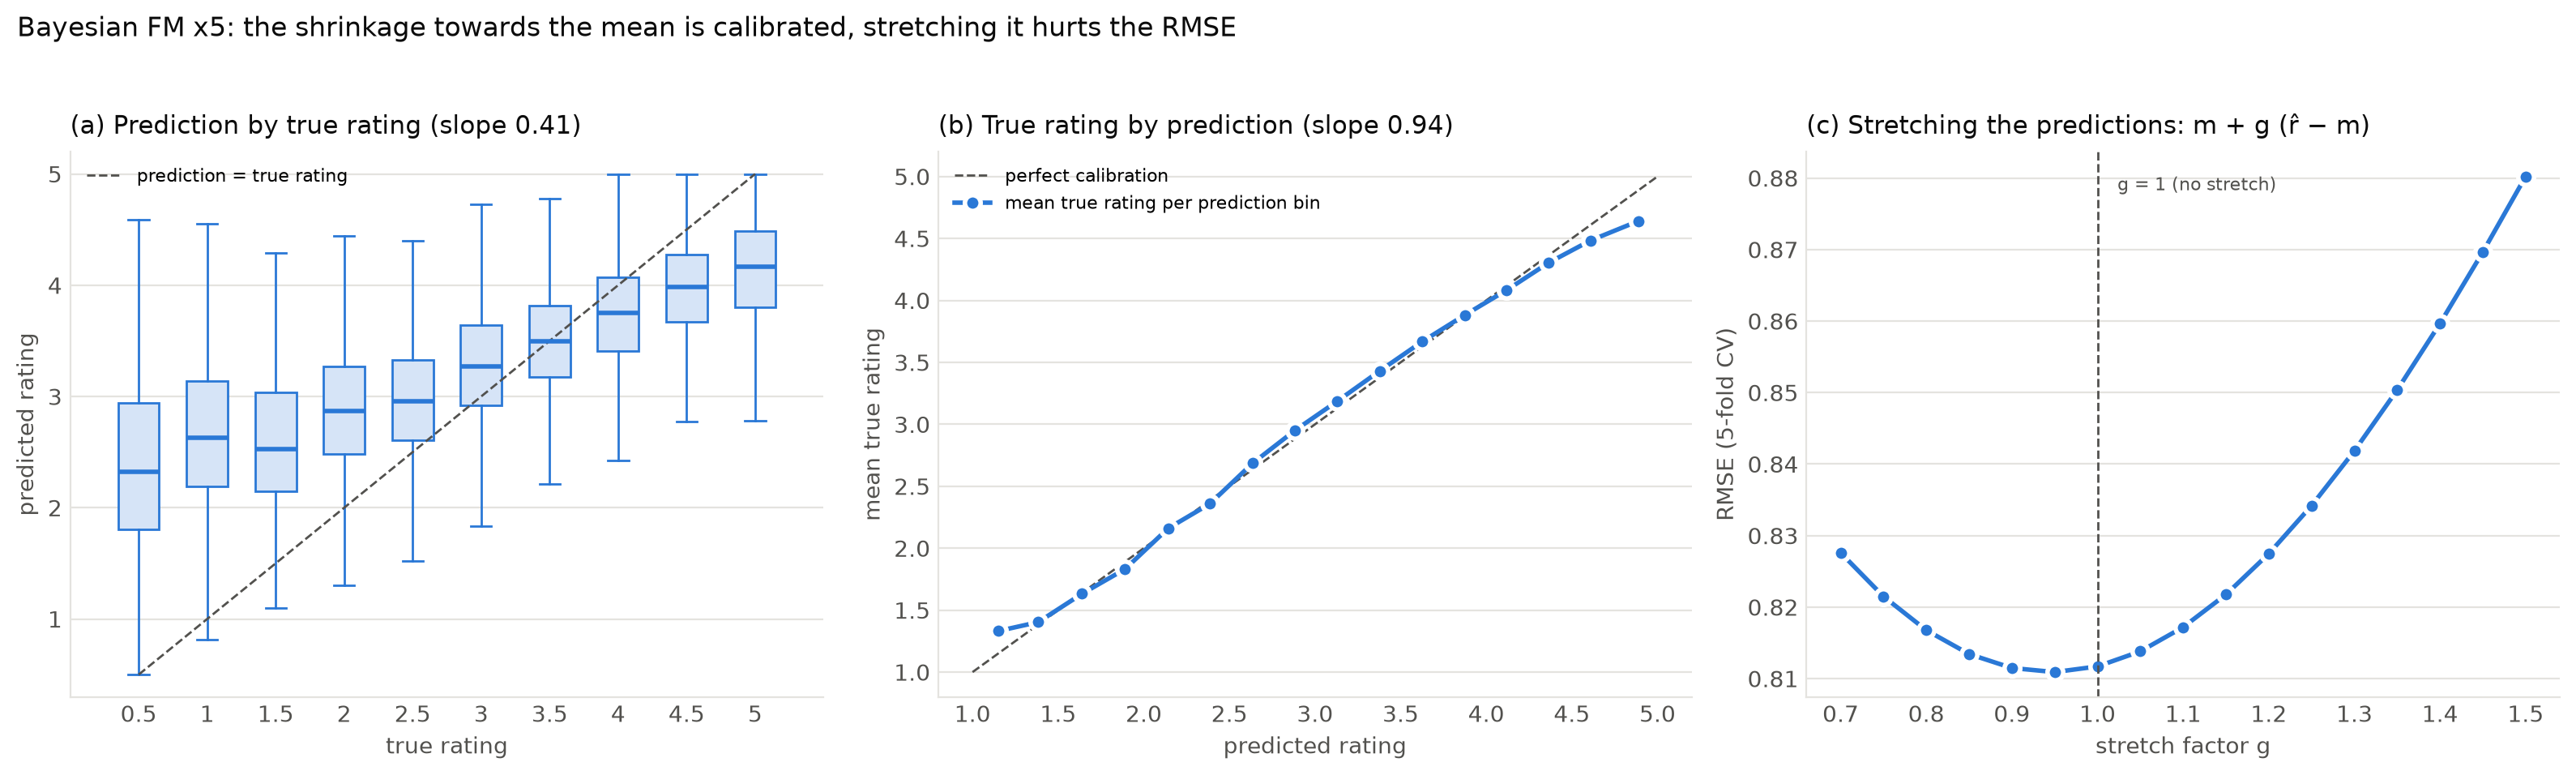
\includegraphics[width=\linewidth]{1a_extremes_calibration.png}
\caption{Bayesian FM $\times 5$, out-of-fold predictions on train $\cup$ test. (a) Prediction against the true
rating. (b) Mean true rating by prediction bin (calibration). (c) CV RMSE after stretching the predictions by $g$.}
\label{fig:calib}
\end{figure}

\subsection{Users with spread-out ratings and user normalization}
Users whose ratings have a standard deviation above 1 account for $31\%$ of the ratings and $46\%$ of the
squared error (Figure~\ref{fig:segments}a). The FM has a single noise level $\alpha^{-1}$ for all users, so a
user who uses the whole scale and a user who only gives 3.5 to 4.5 are fitted with the same confidence. We fit
the FM on normalized ratings $z_{ui} = (r_{ui} - m_u)/s_u$ and map back with $\rhat_{ui} = m_u + s_u \hat z_{ui}$,
where the user mean and standard deviation are shrunk towards the global ones with $\kappa = 20$ pseudo-ratings:
\[
m_u = \frac{\sum_{i\in\Omega_u} r_{ui} + \kappa\mu}{|\Omega_u| + \kappa},\qquad
s_u^2 = \frac{\sum_{i\in\Omega_u} (r_{ui} - m_u)^2 + \kappa\sigma^2}{|\Omega_u| + \kappa}.
\]
The normalization is computed on the training ratings of each fold, so the evaluation set is never used.
The CV RMSE of the FM $\times 5$ goes from $0.8117$ to $0.8049$ ($-0.0068$, on 5 folds out of 5). Every
segment gains, the most spread-out users the most ($-0.015$ for a standard deviation $\ge 1.2$), and so do
the least spread-out ones ($-0.009$), whose narrow scale is now respected.

\subsection{Rarely rated movies}
$18\%$ of the evaluation ratings concern a movie with at most 5 training ratings (Figure~\ref{fig:segments}b).
There, the item kNN is no better than the biases because it has no neighbours to average. The FM is $0.06$ to
$0.09$ better than both, thanks to the genres and to the implicit feedback (who rated the movie). These movies
remain the hardest segment ($0.96$ for unseen movies, against $0.77$ above 50 ratings), and normalization
helps them only slightly.

\begin{figure}[h]
\centering
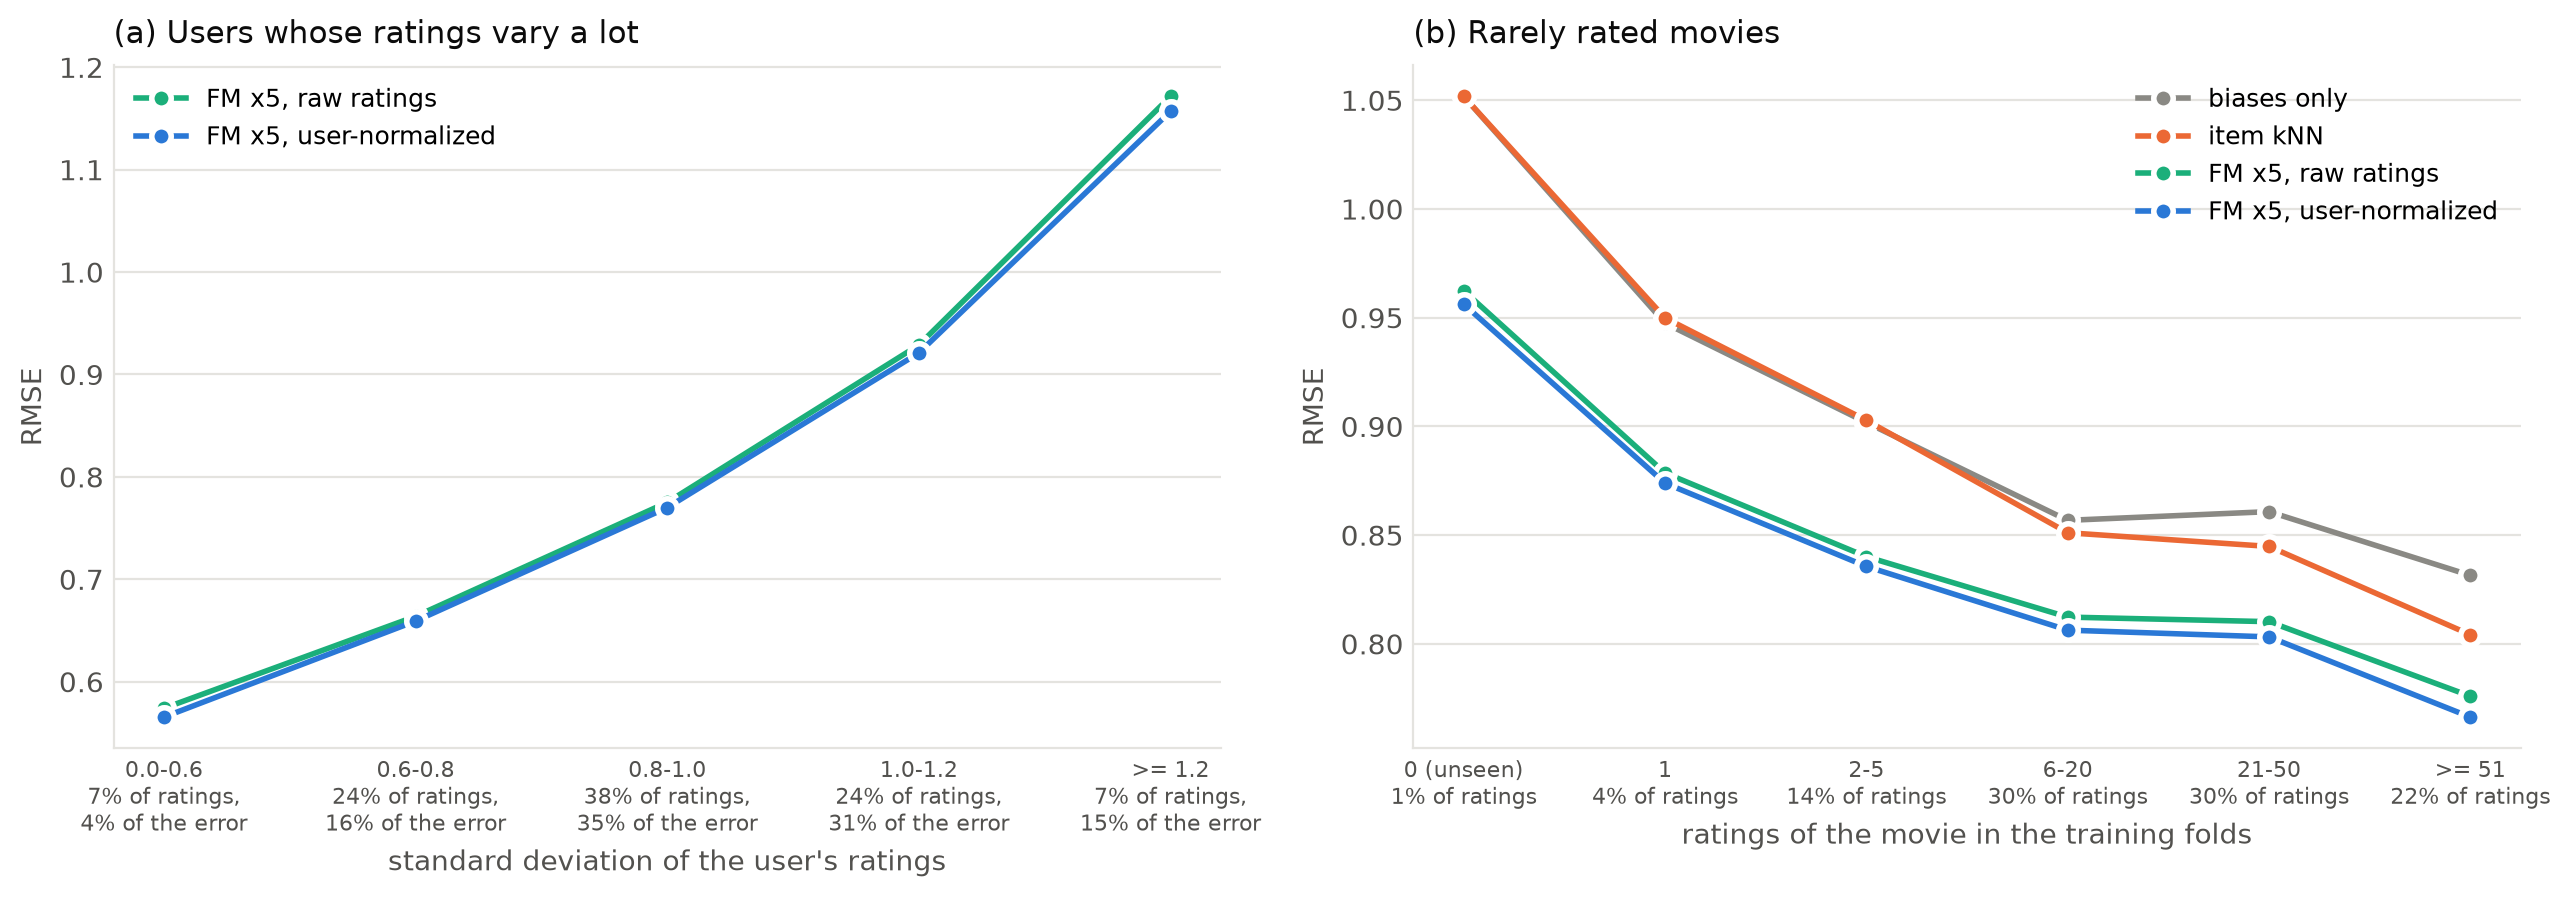
\includegraphics[width=0.85\linewidth]{1bc_users_and_movies.png}
\caption{Out-of-fold RMSE by segment. (a) By standard deviation of the user's ratings, FM $\times 5$ on raw and
normalized ratings. (b) By number of training ratings of the movie: biases, item kNN, FM raw and normalized.}
\label{fig:segments}
\end{figure}

\subsection{Combining the FM with the item kNN}
The two models use different information, latent factors and side features on one side, local co-ratings on
the other. We combined them linearly, $\rhat = w_0 + w_{\text{FM}}\rhat^{\text{FM}} + w_{\text{kNN}}\rhat^{\text{kNN}}$,
with weights fitted by least squares on out-of-fold predictions and evaluated on other folds.

\begin{center}\small
\begin{tabular}{lcccc}
\toprule
 & $w_{\text{FM}}$ / $w_{\text{kNN}}$ & RMSE FM $\to$ stack & error correlation & kNN share of $\Var(\rhat)$ \\
\midrule
raw FM $\times 5$        & 0.821 / 0.161  & $0.8117 \to 0.8098$ & 0.926 & $2.6\%$ \\
normalized FM $\times 5$ & 0.981 / $-0.006$ & $0.8049 \to 0.8048$ & 0.942 & $0\%$ \\
\bottomrule
\end{tabular}
\end{center}

With the raw FM, the kNN brings $-0.0019$, and only where it has neighbours (Figure~\ref{fig:knn}): $-0.003$
on movies with more than 20 ratings and on users with 100 to 300 ratings, while it degrades unseen movies
($+0.0055$), where it only repeats the biases. The errors of the two models are correlated at $0.93$: they fail
on the same ratings, which we expect to be the unpredictable extremes of Section~\ref{sec:extremes}. After normalization the
kNN weight is zero, as the normalization already corrects what the kNN corrected. The raw FM with the kNN was
our submission 3 ($0.801$ on the platform).

\begin{figure}[h]
\centering
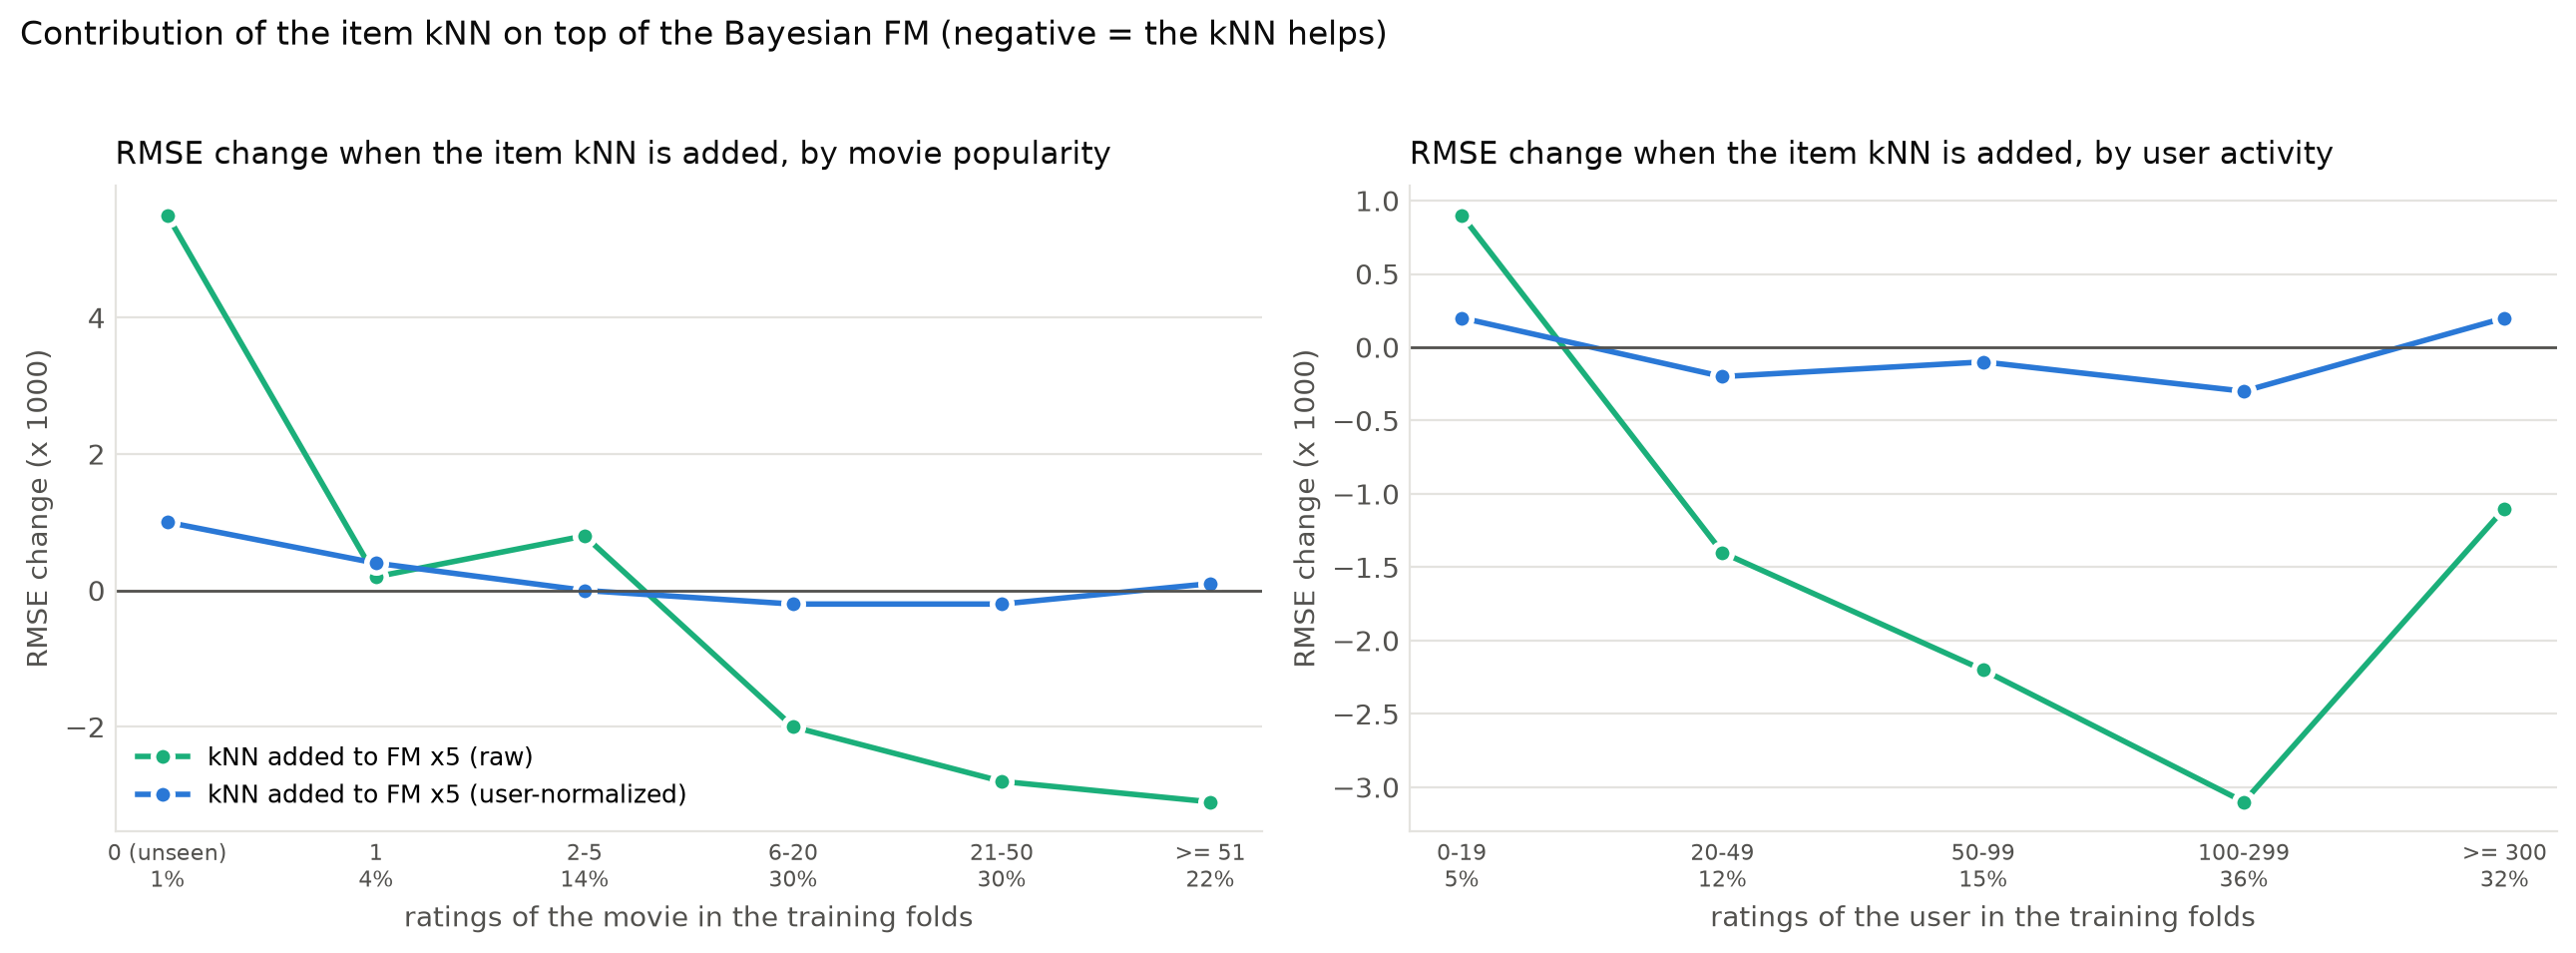
\includegraphics[width=0.85\linewidth]{2_knn_contribution.png}
\caption{RMSE change ($\times 1000$) when the item kNN is added to the FM $\times 5$ in a linear stack, by segment.}
\label{fig:knn}
\end{figure}

\subsection{Gradient boosting on the stack residual}
A linear stack gives the kNN the same weight everywhere, while it is only useful on popular movies. We fit a
gradient-boosted tree model (200 trees, 15 leaves, at least 200 ratings per leaf) on the residual of the linear
stack of the normalized FM, the raw FM and the kNN. Its features are the base predictions, the disagreement
between the 5 chains, the user and movie counts, means and standard deviations, the user's share of half-star
ratings, the genres and the decade. Fitted and evaluated across folds, it brings the CV RMSE to $0.8023$
($-0.0025$ on top of the linear stack, on 5 folds out of 5). This is our final submission; with the observed
gap between CV and platform, we expect about $0.795$.

%% ================================================================ 5
\section{Discussion}

The gains came from averaging over the posterior (BPMF, Bayesian FM, several chains), from side information
on the movies and from user normalization, each holding on every fold. Point-estimate factor models and
neighbourhood models stay within $0.005$ of the biases, stretching the predictions cannot work under RMSE,
and the item kNN adds almost nothing to a normalized FM in a linear combination.

Two limitations remain. The stacking models are trained on out-of-fold predictions of models fitted on $80\%$
of train $\cup$ test, while the submitted base models are fitted on $100\%$, so their predictions are slightly
sharper than those the stack learnt from. The gap between CV and platform ($\approx 0.009$) has been stable over
two submissions only.

At $1\%$ density, the bottleneck is information, not the optimizer: ALS and gradient descent reach the same
minimum, while integrating over the uncertainty and adding information (genres, implicit feedback, per-user
scale) each brought a gain. Hyperparameters must be tuned at the data size of the final fit.

\end{document}
